% 注意：使用 table* 而不是 table
\input{tables/main_results}

\section{Experiments}
\label{sec:exp}

\subsection{Experimental Setup}
\paragraph{Training.}
\label{subsec:sft}
To validate the effectiveness of the synthesized trajectories, we perform supervised fine-tuning (SFT) on a base model initialized from {NVIDIA-Nemotron-3-Nano-30B-A3B-Base-BF16}~\citep{blakeman2025nemotron}. We curate the training data by applying rejection sampling: only trajectories that yield correct final answers are retained, resulting in around 55K trajectories. We adopt {Megatron-LM}~\citep{megatron-lm} as the distributed training framework. All experiments follow a fixed and controlled configuration to ensure reproducibility. Training is conducted on 8 NVIDIA H100 GPUs for approximately 8 hours, with a learning rate of $5\times10^{-5}$ without learning rate decay. To accommodate the long-horizon nature of our trajectories, sequences are pre-packed to a maximum context length of 256K tokens, eliminating truncation artifacts and preserving complete reasoning chains. The training process runs for 347 steps with a global batch size of 64.
% \yz{Do you have an easy-to-justify reason for training only one epoch?}

This configuration enables the model to directly internalize extended tool-use patterns, multi-step evidence aggregation, and adaptive search strategies from full-length trajectories. By learning from untruncated, answer-verified demonstrations, the model acquires the capacity to plan and execute complex web-scale reasoning tasks without relying on heuristic shortcuts or premature termination.

\paragraph{Evaluation. }
\label{sec:exp-setup} To comprehensively evaluate capabilities of \model, 
we consider a suite of deep research benchmarks, including: (1) \textit{Closed-web search}: BrowseComp-Plus~\citep{chen2025BrowseCompPlus}; (2) \textit{Open-web search}: BrowseComp~\citep{wei2025browsecomp}, GAIA~\citep{mialon2023gaia}, and xbench-DeepSearch~\citep{chen2025xbench}. For BrowseComp-Plus, we use the officially released corpus together with a Qwen3-Embedding-8B FAISS index to construct the offline search engine. The remaining open-web benchmarks rely on the Serper API~\citep{serperdev2026} for online search. This evaluation setup allows us to test both: in-corpus reasoning ability under fully reproducible conditions, and generalization to real-world web search environments. More evaluation details are provided in Appendix \S\ref{app:eval_details}.

\paragraph{Baselines.}
We include two categories of baselines: (1) \textit{Foundation Models with Tools}: GPT-4.1~\citep{openai2025gpt41}, Claude-4-Opus~\citep{anthropic2025claude4opus},  Claude-4-Sonnet~\citep{anthropic2025claude4opus},  Gemini-2.5-Pro~\citep{comanici2025gemini25},  Kimi-K2~\citep{team2025kimi},  DeepSeek-R1~\citep{guo2025deepseekr1},  DeepSeek-R1~\citep{liu2024deepseekv3},  Nemotron-3-Nano-30B-A3B~\citep{blakeman2025nemotron}, and OpenAI o4-mini~\citep{openai2025o4mini}. (2) \textit{DeepResearch Agents}: 
Tongyi DeepResearch~\citep{team2025tongyideepresearch},  CutBill~\citep{wu2025cutthebill}, ASearcher~\citep{gao2025Asearcher},  WebDancer~\citep{wu2025webdancer},  WebSailor~\citep{li2025websailor}, and DeepMiner~\citep{tang2025deepminer}.  More details on baseline implementations are in Appendix \S\ref{app:baselines}.

\subsection{Main Results}
\label{sec:main_results}

\paragraph{Key Insights.} Table~\ref{tab:main_results} summarize our main results. We highlight two key observations: (1) \textit{BrowseComp-Plus.} Our \model-30B-A3B achieves \textbf{54.8\% accuracy} on this benchmark, substantially outperforming strong proprietary baselines including GPT-4.1 (36.4\%), Claude-4-Opus (36.8\%), and DeepSeek-R1 (16.4\%). This corresponds to a \textbf{+34.0\% absolute improvement} over the base Nemotron-3-Nano-30B-A3B model (20.8\%). These results indicate that SFT on synthesized long-horizon trajectories alone is sufficient to unlock significant gains in deep-research performance, even without reinforcement learning or additional online interaction. (2) \textit{Open-Web Deep Research Benchmarks.} We further evaluate generalization to real-world search environments using the three benchmarks that rely on live web search APIs, where \model-30B-A3B achieves \textbf{26.3\%}, \textbf{64.1\%}, and \textbf{65.0\%} accuracy on BrowseComp, GAIA, and xbench-DeepSearch, respectively. 
These results remain competitive with strong frontier models, while substantially outperforming existing open-source deep research systems, including ASearcher-QwQ-32B (5.2\%/52.8\%/42.0\%) and WebDancer-QwQ-32B (3.8\%/51.5\%/39.0\%). 
Crucially, these gains are achieved \textbf{without any training on live web data}---our model is fine-tuned solely on trajectories synthesized in the offline environment. 
This demonstrates that high-quality, reproducible offline synthesis can produce training signals that generalize effectively to dynamic, real-world search environments.


\subsection{In-Depth Analysis of 97K+ Deep-Research Trajectories}
\label{subsec:trajectory_statistics}

\begin{figure*}[t]
    \centering
    \vspace{-0.5em}
    % --- 右图 ---
    \begin{minipage}[b]{0.68\textwidth}
        \centering
        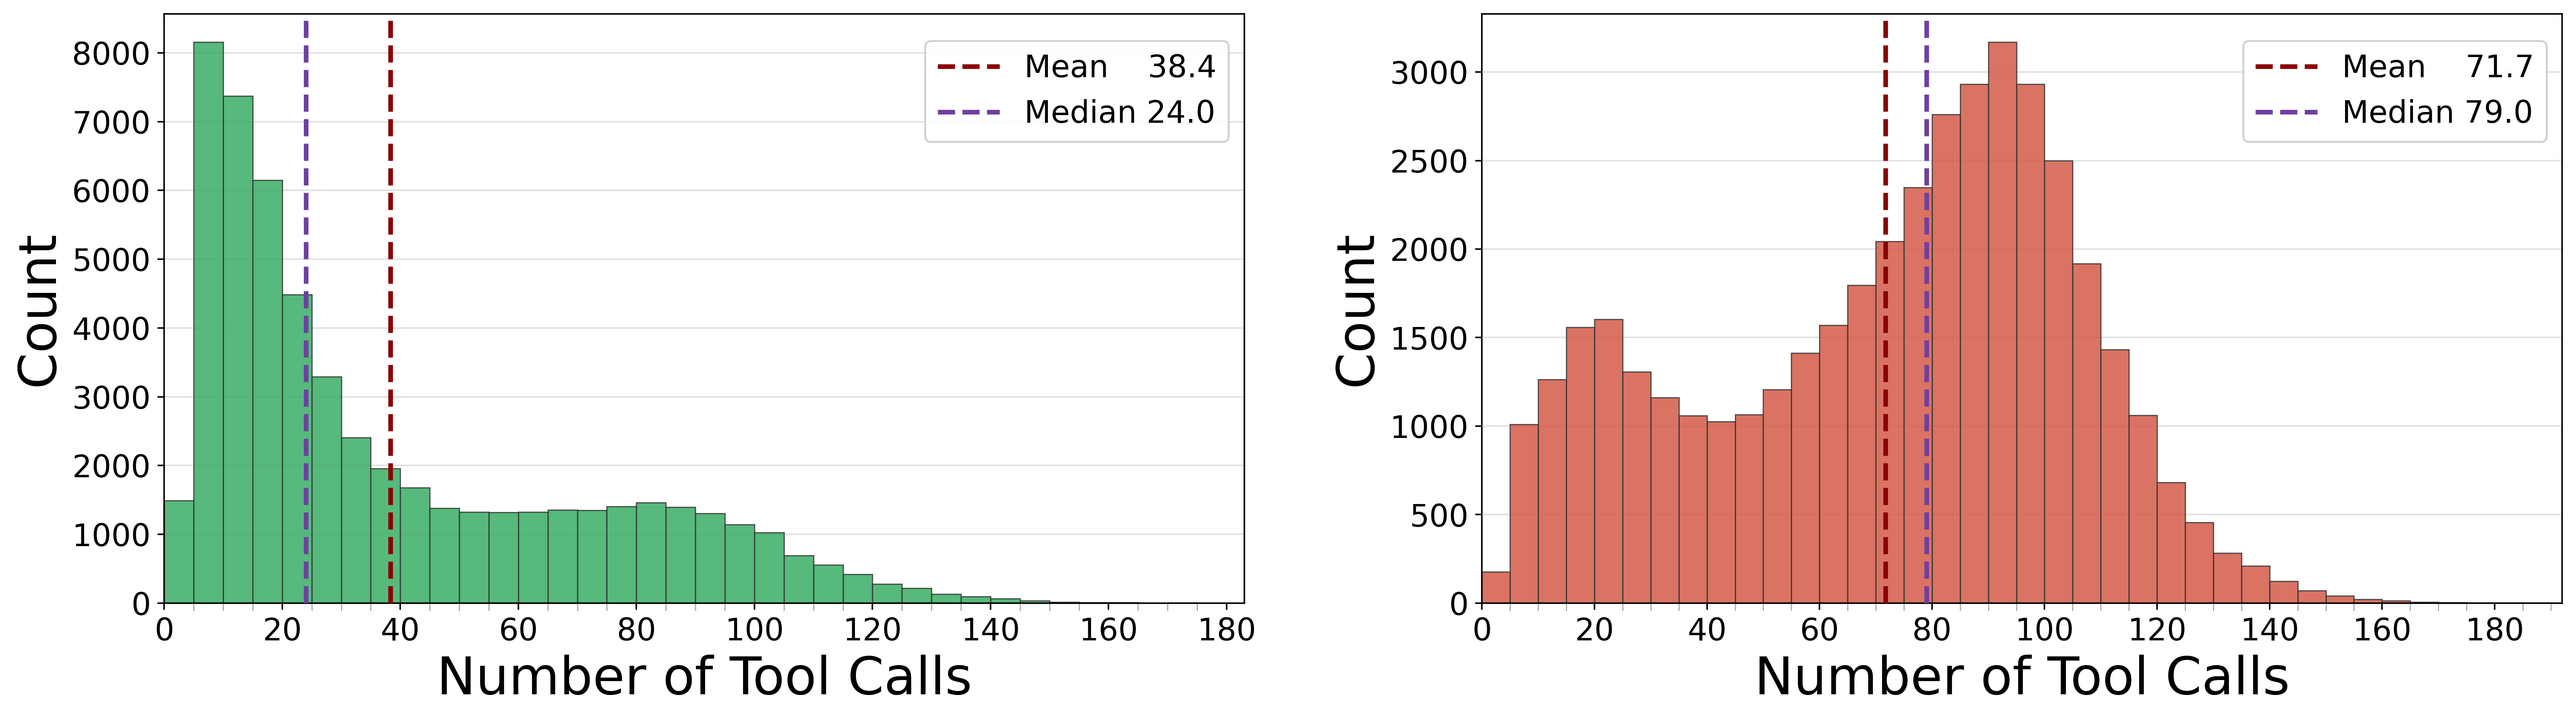
\includegraphics[width=\linewidth]{img/turn_distribution.png}
    \end{minipage}
    \hfill
    % --- 右图 ---
    \raisebox{0.25em}{%
    \begin{minipage}[b]{0.3\textwidth}
        \centering
        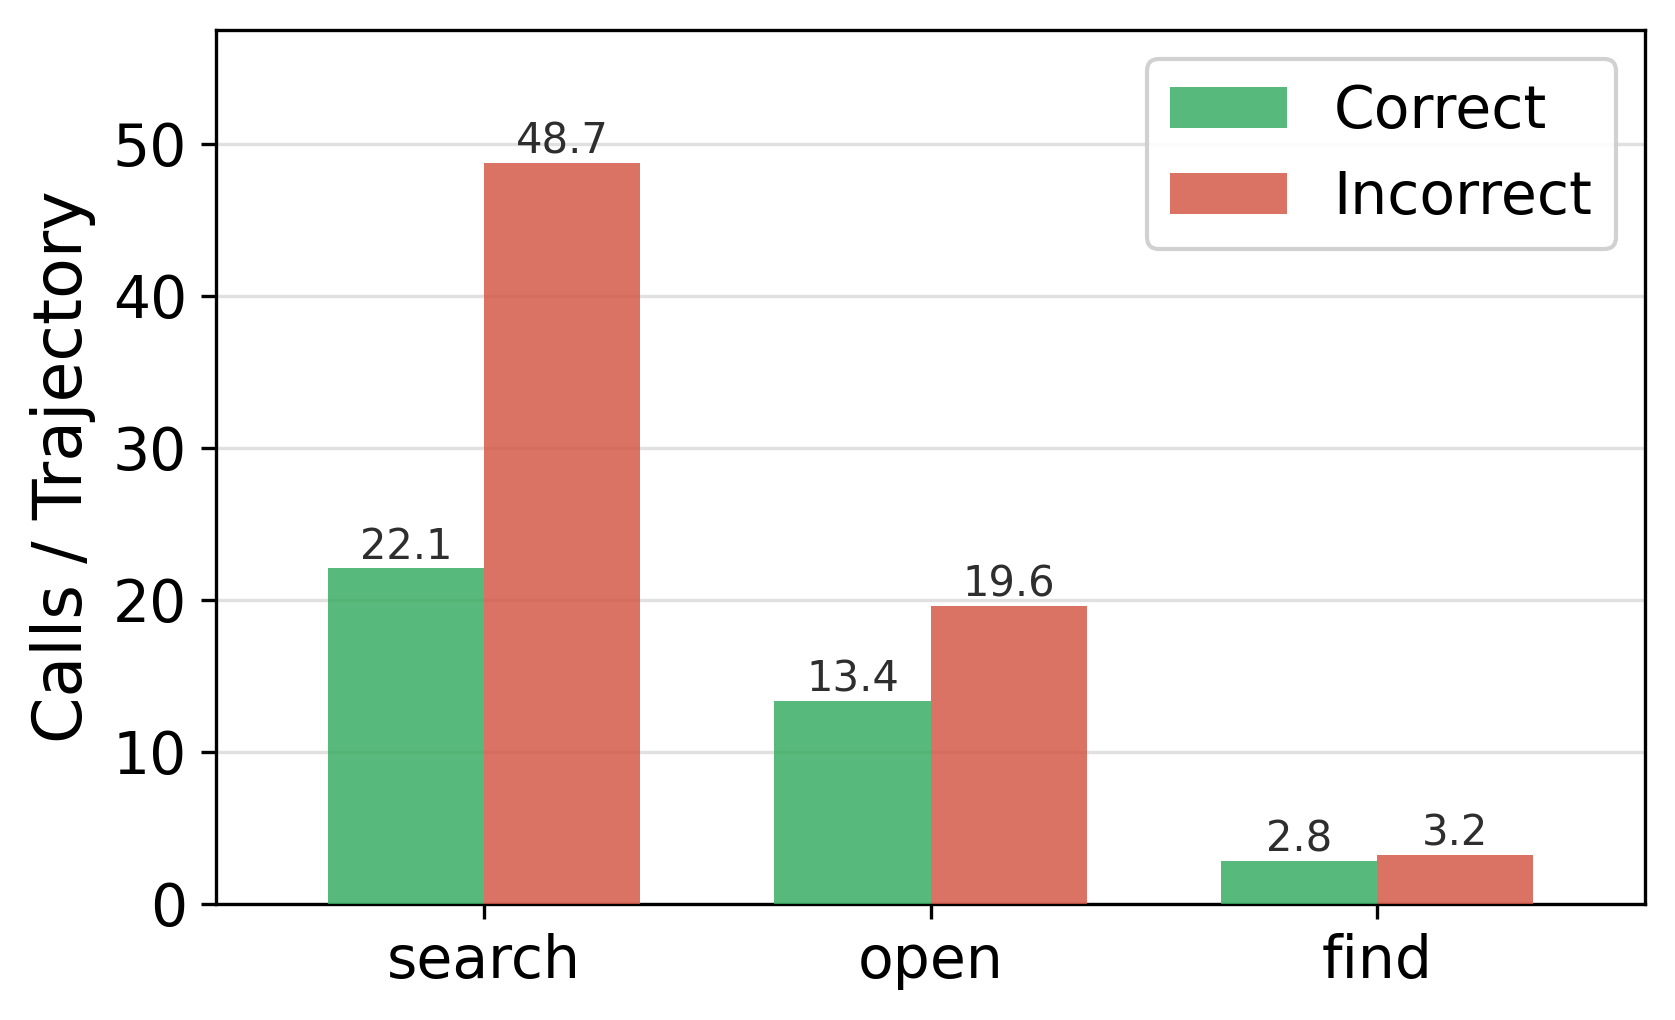
\includegraphics[width=\textwidth]{img/tool_usage.png}
    \end{minipage}}
    \vspace{-0.5em}
    \caption{
    (Left, Middle) Distribution of tool-call counts per trajectory with bin width 5. (Right) Average tool usage across \texttt{search}, \texttt{open}, and \texttt{find}, split by correct and incorrect outcomes.
    % Distribution of tool-call counts per trajectory (bin width = 5) (Lefe and Middle) and average tool usage across \texttt{search}, \texttt{open}, and \texttt{find} (Right), by correct and incorrect outcomes.
    % Distribution of tool-call counts per trajectory (bin width=5), split by outcome. Dashed/dotted lines mark the mean/median. (Left) Correct trajectories are right-skewed. (Middle) Incorrect trajectories exhibit a bimodal distribution with peaks near 20 and 90. The $3{\times}$ higher median suggests failures either terminate early or exhaust the budget without converging. (Right) Average tool usage statistic on all synthesis trajectories. \todo{update} 
    }
    \vspace{-1em}
    \label{fig:turn-distrib}
\end{figure*}

% Following standard practice~\citep{touvron2023llama,jiang2024mixtral}, 
% we apply rejection sampling to retain only successful trajectories for downstream supervised fine-tuning. 
% Here we provide a deeper analysis of the resulting 97K long-horizon deep-research trajectories.

\label{subsec:success_rate}
\input{tables/trajectory_stats}

\paragraph{Overall Success Rate and Tool Usage.}

Table~\ref{tab:trajectory_stats} summarizes key statistics of the synthesized trajectories. A notable observation is the large disparity in tool usage between correct and incorrect trajectories, measured by the total number of calls to \texttt{search}, \texttt{open}, and \texttt{find}. Failed trajectories require nearly twice as many tool calls on average (71.7 vs.\ 38.4). This suggests that failure stems not from insufficient exploration, but rather from \textit{inefficient or misdirected search strategies} on hard cases. To mitigate this, harder questions demand better search mechanisms rather than simply more steps. The distribution of tool-call counts in Figure~\ref{fig:turn-distrib} (left, middle) further supports this observation. As shown in the left panel, successful trajectories are concentrated in the 10 to 40 tool-call range, indicating that many queries can be resolved with relatively efficient reasoning. In contrast, the middle panel shows that failed trajectories follow a broader, bimodal distribution with a substantially higher median (79.0 vs. 24.0), suggesting repeated search attempts without convergence. Nevertheless, a non-trivial portion of successful trajectories still exceeds 100 tool calls, with some reaching the maximum horizon. This wide spectrum also ensures that downstream models are exposed to both concise and complex reasoning patterns, mitigating the risk of learning shallow retrieval shortcuts. 

\paragraph{Tool Call Distribution.}
We further analyze tool usage across the three primitives (\texttt{search}, \texttt{open}, and \texttt{find}) in Figure~\ref{fig:turn-distrib} (right). The results indicate that the excess tool calls in failed trajectories are primarily driven by \texttt{search} operations, which account for the majority of the disparity (48.7 vs. 22.1 calls). While \texttt{find} usage remains similar across outcomes (3.2 vs. 2.8), \texttt{open} calls are also moderately higher in failed trajectories (19.6 vs. 13.4). This pattern implies that successful trajectories tend to converge on relevant documents earlier, while failed ones repeatedly reformulate queries without making grounded progress. In other words, document-level navigation is not the primary bottleneck; rather, query formulation and search drift drive the performance gap. This finding aligns with our motivation for designing explicit browser primitives to address search inefficiencies.

\paragraph{Pass@$k$ Analysis.}
\begin{wrapfigure}{r}{0.58\textwidth}
    \vspace{-1em}
    \centering
    % --- 左图 ---
    \begin{minipage}[b]{0.49\linewidth}
    \centering
        \includegraphics[width=\linewidth]{img/passatk_bar.png}
    \end{minipage}
    \hfill
    % --- 右图（向下调整）---
    \begin{minipage}[b]{0.49\linewidth}
        \centering
        \raisebox{0em}{
        \includegraphics[width=\linewidth]{img/passrate_distribution.png}}
    \end{minipage}
    \vspace{-1em}
    \caption{(Left) Pass@$k$ comparison. (Right) Solve rate distribution on all unique queries.}
    \vspace{-1.5em}
    \label{fig:combined-stats}
\end{wrapfigure}
To measure solution diversity, we compute Pass@$k$ over the 16 sampled trajectories per question (Figure~\ref{fig:combined-stats}, left). Pass@1 is 0.567 and steadily increases to 0.792 at Pass@16. This 20\%+ gap suggests that many questions are solvable, but only along certain reasoning paths. Moreover, the solve-rate distribution is highly skewed. Per-question analysis reveals a bimodal pattern (Figure~\ref{fig:combined-stats}, right; mean=0.567, median=0.688): a significant portion (over 20\%) of questions have a pass rate near 0\%, representing extremely hard cases, while another substantial portion (approximately 30\%) reaches near 100\%, indicating robust solvability. The remaining questions fall in the intermediate range and constitute the main space for improvement. This structure is characteristic of open-ended, web-scale research tasks, where success often hinges on discovering a small set of critical facts. More statistics on Pass@$k \in\{1,2,3,4,8,16\}$ are provided in Appendix \S\ref{app:exp_traj}. 



\subsection{Cost Efficiency of Offline Synthesis}
\label{subsec:cost_analysis}
\input{tables/cost_comparison}
A major motivation for our offline search design is scalability. 
Table~\ref{tab:cost_comparison} compares the estimated cost of synthesizing our 97K+ trajectories (with 5.76M search requests) using online APIs versus our offline retriever. Beyond direct cost savings, our offline design offers three additional advantages: 
(1) \textbf{no rate limits}, enabling parallel synthesis at scale; 
(2) \textbf{fully deterministic behavior}, ensuring perfect reproducibility across runs; and 
(3) \textbf{zero dependency on proprietary infrastructure}, facilitating open dissemination. 
Together, these properties make large-scale, long-horizon trajectory synthesis feasible for the first time in a fully open setting.


\subsection{Ablation Study and Discussion}
\label{subsec:ablation}
\input{tables/rq1_rq2_combined}

\paragraph{RQ1: Is final-answer correctness a necessary filtering signal for trajectory SFT?} \label{subsec:ablation_rq1} A striking yet important observation from deep research is that final-answer correctness alone is not the dominant indicator of training value. Even failed trajectories provide useful supervision about search structure, tool-use order, evidence inspection, and stopping behavior. To test this, we keep the student backbone, optimization recipe, and evaluation protocol fixed, varying only which synthesized trajectories are used for SFT. The left half of Table~\ref{tab:rq1_rq2} shows that training on correct-only (54.81\%), incorrect-only (55.06\%), and mixed trajectories (54.46\%) yields nearly identical downstream accuracy on BrowseComp-Plus, with all three settings within 0.6 percentage points. We therefore avoid over-interpreting their exact ranking.

\paragraph{RQ2: Is one-time online bootstrapping for corpus coverage necessary for effective offline synthesis?} \label{subsec:ablation_rq2}
One-time online bootstrapping is critical for effective offline synthesis because corpus coverage is a hard prerequisite for meaningful search trajectories. For this targeted corpus-coverage ablation, we rerun synthesis on the 6K-prompt corpus-construction split with 4 seeds per prompt, comparing the standard corpus against a variant without bootstrapped gold documents. The right half of Table~\ref{tab:rq1_rq2} shows a severe degradation at both synthesis time and downstream evaluation: removing gold documents drops the gold-document hit rate from 29.54\% to 1.73\%, lowers trajectory accuracy from 56.86\% to 43.81\%, and collapses downstream BrowseComp-Plus accuracy from 54.81\% to 6.35\%. This is not a marginal effect. It shows that one-time online bootstrapping is not merely helpful but essential for constructing an offline corpus that supports effective trajectory synthesis and downstream post-training.

\input{tables/max_turn_wrap}
\paragraph{RQ3: How much turn budget is enough for BrowseComp-Plus?} \label{subsec:ablation_rq3}
Holding the model, prompt, and corpus fixed, we sweep the maximum allowed turn budget on BrowseComp-Plus. Figure~\ref{fig:rq3_max_turn_budget} shows that both ACC and gold hit rate improve steadily as the budget increases, then begin to plateau beyond roughly 100 turns. This indicates that long-horizon exploration is genuinely beneficial, but simply extending the horizon yields diminishing returns once the agent has sufficient opportunity to locate and inspect the relevant evidence.

\input{tables/rq4_rq5_combined}

\paragraph{RQ4: Do explicit browser tools matter for realistic deep research?} \label{subsec:ablation_rq4}
Yes. We test this claim with a teacher-side ablation using GPT-OSS-120B, keeping the model, prompt, and retrieval backend fixed while varying the available browser tools at inference time. The left half of Table~\ref{tab:rq4_rq5} shows a clear progression. \texttt{search}-only performs poorly on all metrics, reaching just 43.86\% accuracy with a 1.45\% gold-document hit rate. Adding \texttt{open} produces the largest jump, improving accuracy to 56.39\% and making evidence access substantially more reliable. Adding \texttt{find} on top of \texttt{search+open} further improves accuracy to 62.17\%, raises the gold-document hit rate to 53.37\%, moves the first gold hit earlier (20.60 to 17.23 turns), and reduces both tool calls and average token usage. These results support the full browser abstraction: document access is necessary, and in-page evidence localization provides additional gains even after retrieval succeeds.

\paragraph{RQ5: Does retrieving gold documents guarantee a correct final answer?} \label{subsec:ablation_rq5}
No. The right half of Table~\ref{tab:rq4_rq5} shows that merely surfacing a gold document in search results is much weaker than explicitly opening it: $P(\text{correct}\mid\text{search-hit})$ is 61.84\%, whereas $P(\text{correct}\mid\text{open-hit})$ rises to 86.72\%. At the same time, nearly all correct trajectories involve gold-evidence exposure, with $P(\text{search-hit}\mid\text{correct})=99.38\%$ and $P(\text{open-hit}\mid\text{correct})=95.01\%$. Figure~\ref{fig:rq5_open_hit_heatmap} shows the same pattern from another angle: trajectories with no gold-document open-hit are overwhelmingly low-accuracy (7.9\%, $n=303$), whereas trajectories with at least one opened gold document maintain consistently high accuracy across a broad range of hit turns. Together, these results distinguish retrieval failure from reasoning failure: evidence exposure is usually necessary, but it does not by itself guarantee a correct final answer.

\input{tables/rq3_open_hit_heatmap}
